%!TEX root = main.tex
\chapter{Pose Estimation}\label{chapter:pose_estimation}
\section{Overview}\label{sec:pose_estimation_overview}
As already mentioned in introduction, estimating the pose of camera (also called tracking) is a crucial part in most computer vision applications. In the case of augmented reality applications, currently two approaches have been used: marker-based pose estimation and feature-based pose estimation. In both approaches, the pose estimator tries to make an estimation of camera relative to the scene. Also there are many techniques for both approaches as explained in previous sections. \\
The main point of this thesis is to add one efficient and precise feature-based pose estimation approach to the Ubitrack framework. To reach this goal, some necessary algorithms such as robust feature matching and bundle adjustment were developed and added to Ubitrack. In this section, the mechanism of a novel feature-based pose estimation based on robust feature matching and bundle adjustment will be described in detail. Similar to most new techniques for SLAM, SfM, and tracking topics in computer vision, this task also is divided into two phases: tracking and mapping. The whole procedures for each phase will be explained individually, and at the end the pose estimation based on the tracking and mapping phases will be described. Better understanding of tracking phases, requires some background knowledge that are described in the following sections.

\subsection{Pose estimation by tracking plane}\label{subsec:pose_estimation_planer_tracking}
Pose estimation by tracking plane is one of the well-known methods for pose estimation, based on the feature points proposed by Gilles Simon et.al \cite{genc2002marker}. This method is justified by the fact that there are some rectangular structures such as ground plane, walls, buildings, etc that are visible in the image. At the first, the homography matrix $H_{w}^{0}$ is estimated by several correspondence points which can be given by hand between the first image and 3D world. This matrix is the mapping between the first image (virtual) and the world (real). After that, the method tries to make a homography matrix between the first image and the next one that both of them have the same plane. This pose estimation method is relied on changing of the homographies that can be retrieved by the relation between the plane and a frame of the sequence. This method assumes the homography matrix $H_{t-1}^{t}$ is a map between the frame at time t-1 and the frame at time t that can be computed by the four points matches between them. The final homography that is the relation between the frame at time t and world plane can be estimated by chaining the successive transformation, which can be written as:
\begin{gather*}
	H_{w}^{t} = H_{t-1}^{t} H_{t-2}^{t-1} \cdots H_{0}^{1} H_{w}^{0}
\end{gather*}\label{eq:homography_world_to_refrence}

% TODO: check the homography
% TODO: add image 
In this thesis, we use of this technique to compute an initial pose estimation for each frame of input sequence, where the pose of first camera is taken from the reference system. As the homography matrix uses the SVD method for computing, the result has error due to the noise in input images or for the wide base-line images. To overcome this problem, all homographies are computed in two steps. First, an approximation of homography is estimated by the matching feature points between two images. Then the following image is warped by this homography so that it is roughly aligned with the reference image. Second, the new small baseline homography is computed again but for the warped image and reference image. The multiplication of the first and second homographies computes an accurate and final homography between the images.
\subsection{Computation of homography matrix from the reference projective matrix}
Sometimes, especially for the first frame, the reference homography or $H_{w}^{0}$ that is a mapping between the first image and the world is necessary. Usually, for the beginning of feature tracking, we use a reference system. A projective matrix has been taken by the reference system that should be converted into the correspondence homography matrix. For this purpose, we assume the projective matrix $P$ can project all 3D points on the $z=0$ plane that has the form $X=(x,y,0,1)$ into the first image. So we have:
\begin{align*} 
x  &=  P X \\
   &=  K [r_{1}r_{2}r_{3}t] 
 \begin{pmatrix}
  X \\
  Y \\
  0 \\
  1
 \end{pmatrix} \\
  &=  K [r_{1}r_{2}t] \begin{pmatrix}
  X \\
  Y \\
  1
 \end{pmatrix} \\
  &=  H_{w}^{0} \begin{pmatrix}
  X \\
  Y \\
  1
 \end{pmatrix} \\
\end{align*}
And therefor we have:
\begin{gather*}
	H_{w}^{0} = K [r_{1}r_{2}t]
\end{gather*}\label{eq:homography_to_projective}

\subsection{Implementation of pose estimation based on planner tracking}
% TODO: describe
The data flow of our pose estimation module will be shown in \autoref{fig:pose_estimation}.

\begin{figure}[H]
\begin{tabular}{cc}
  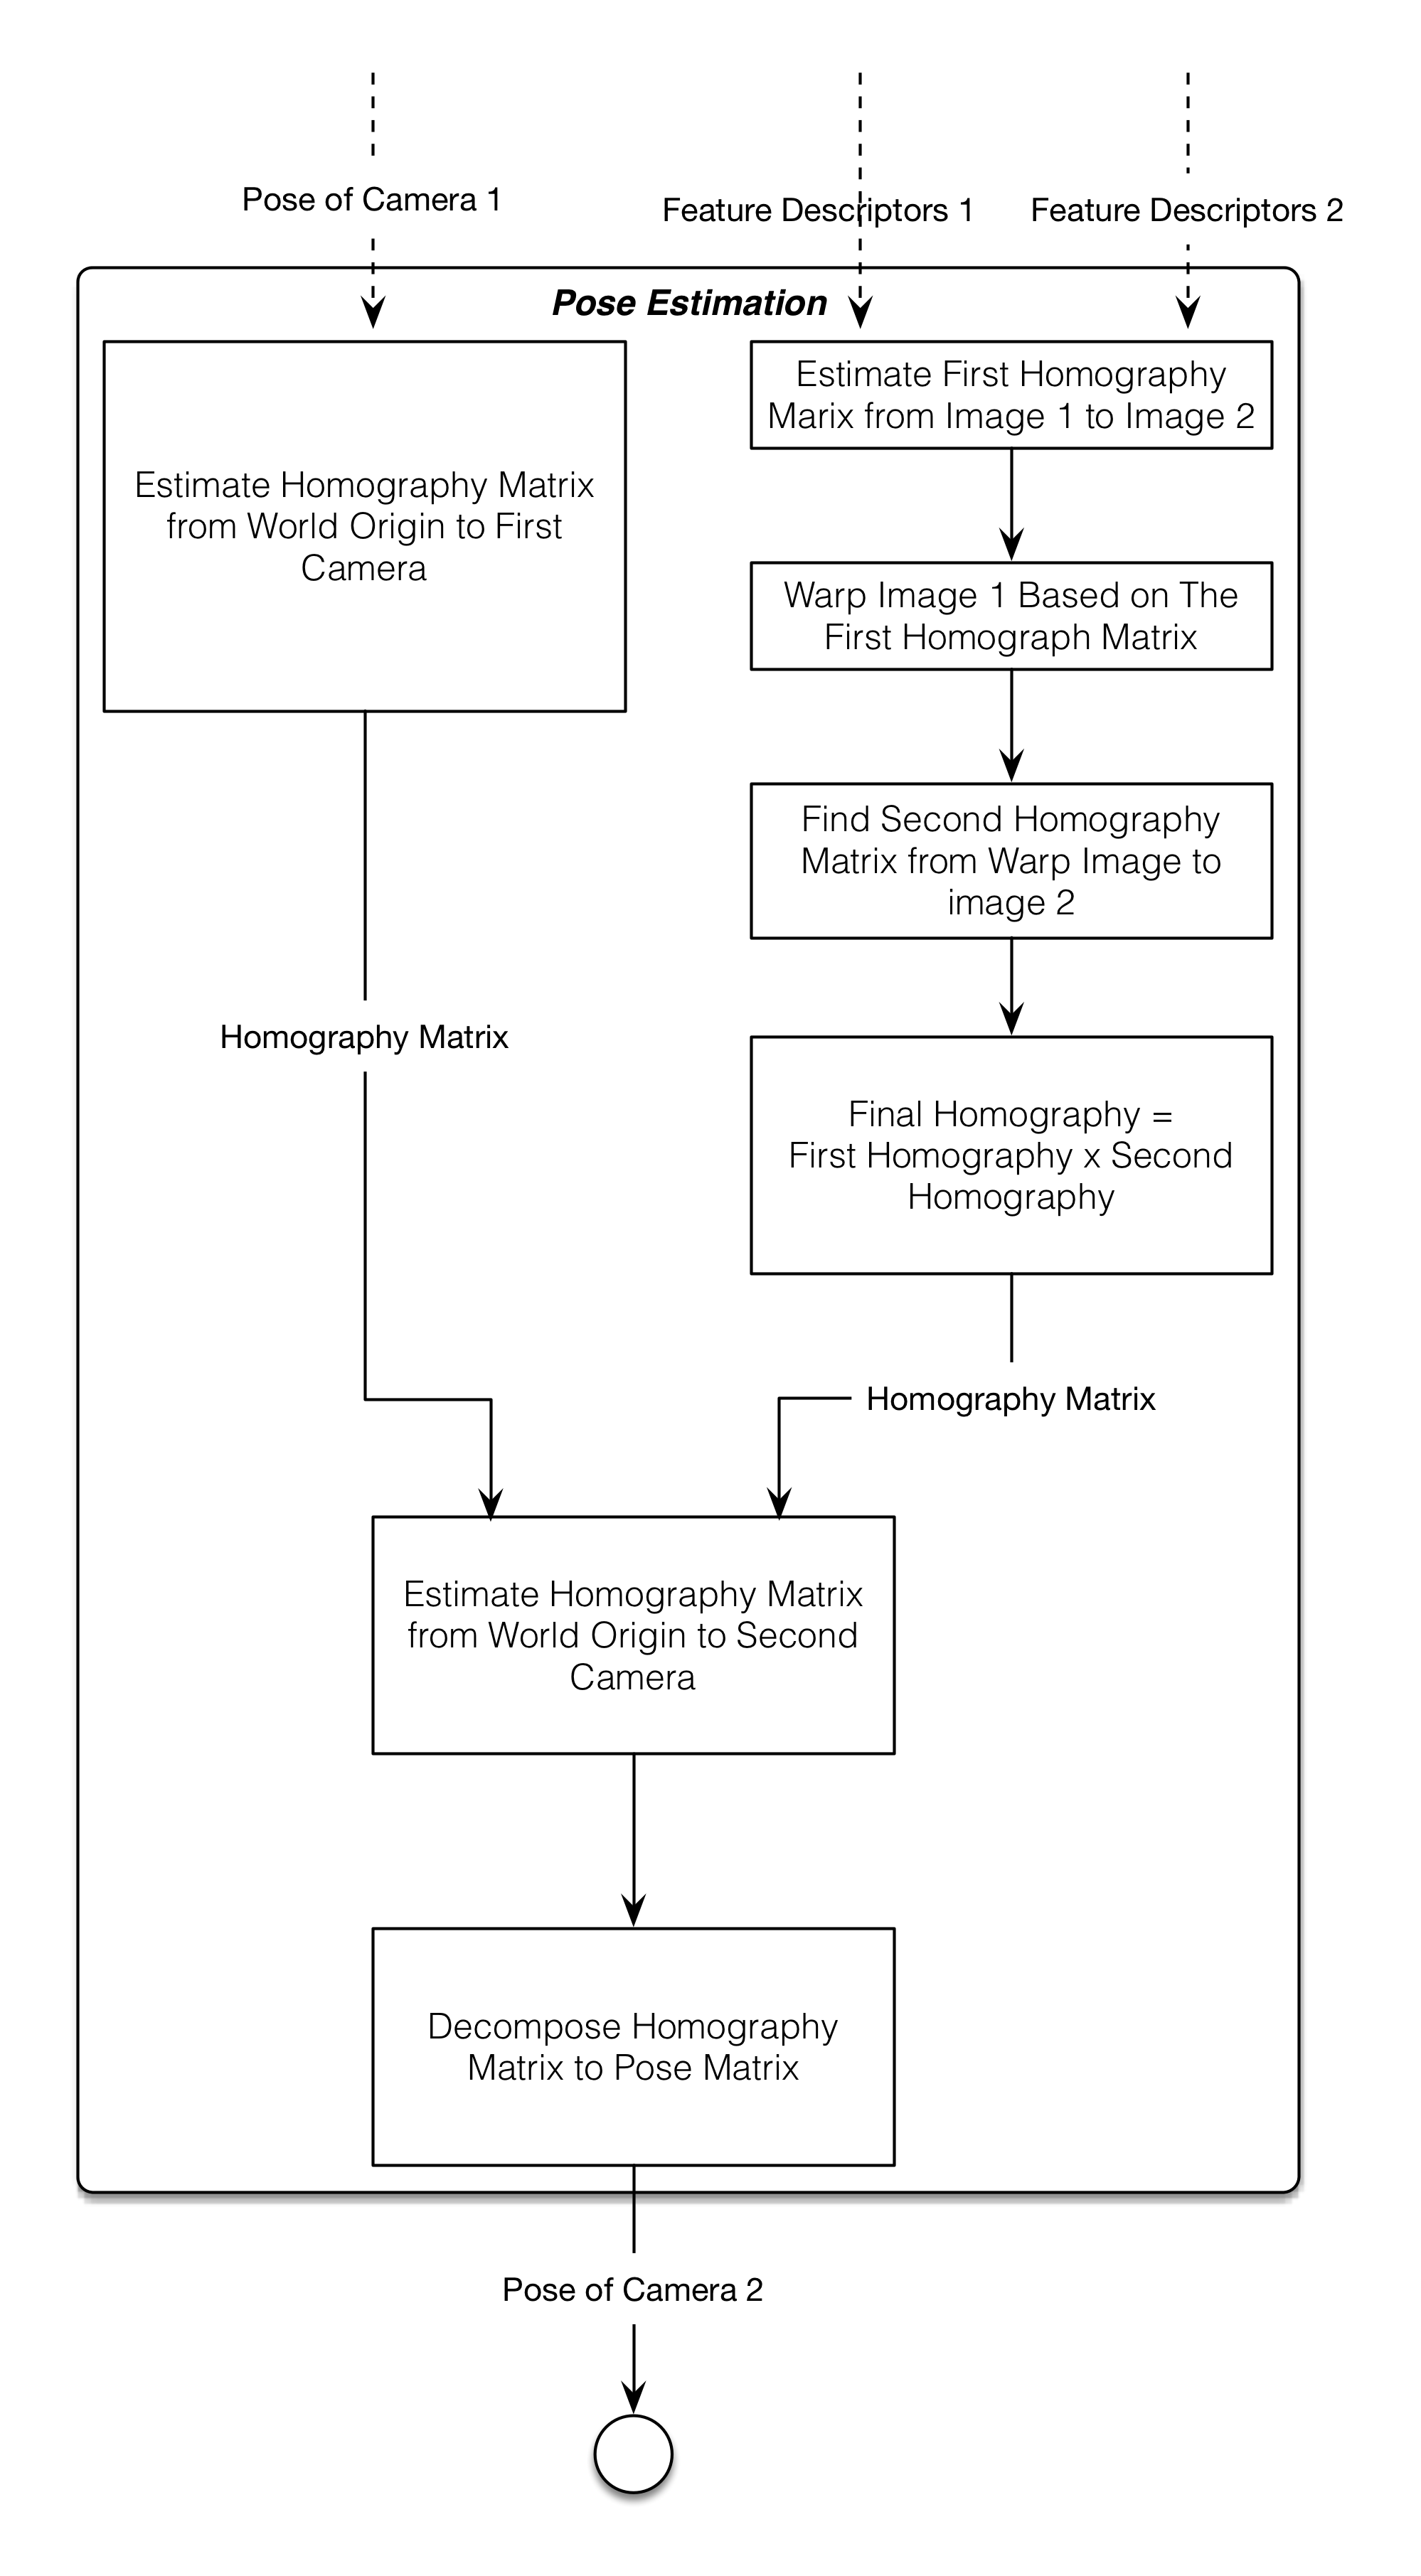
\includegraphics[width=75mm]{figures/pose_estimation} &  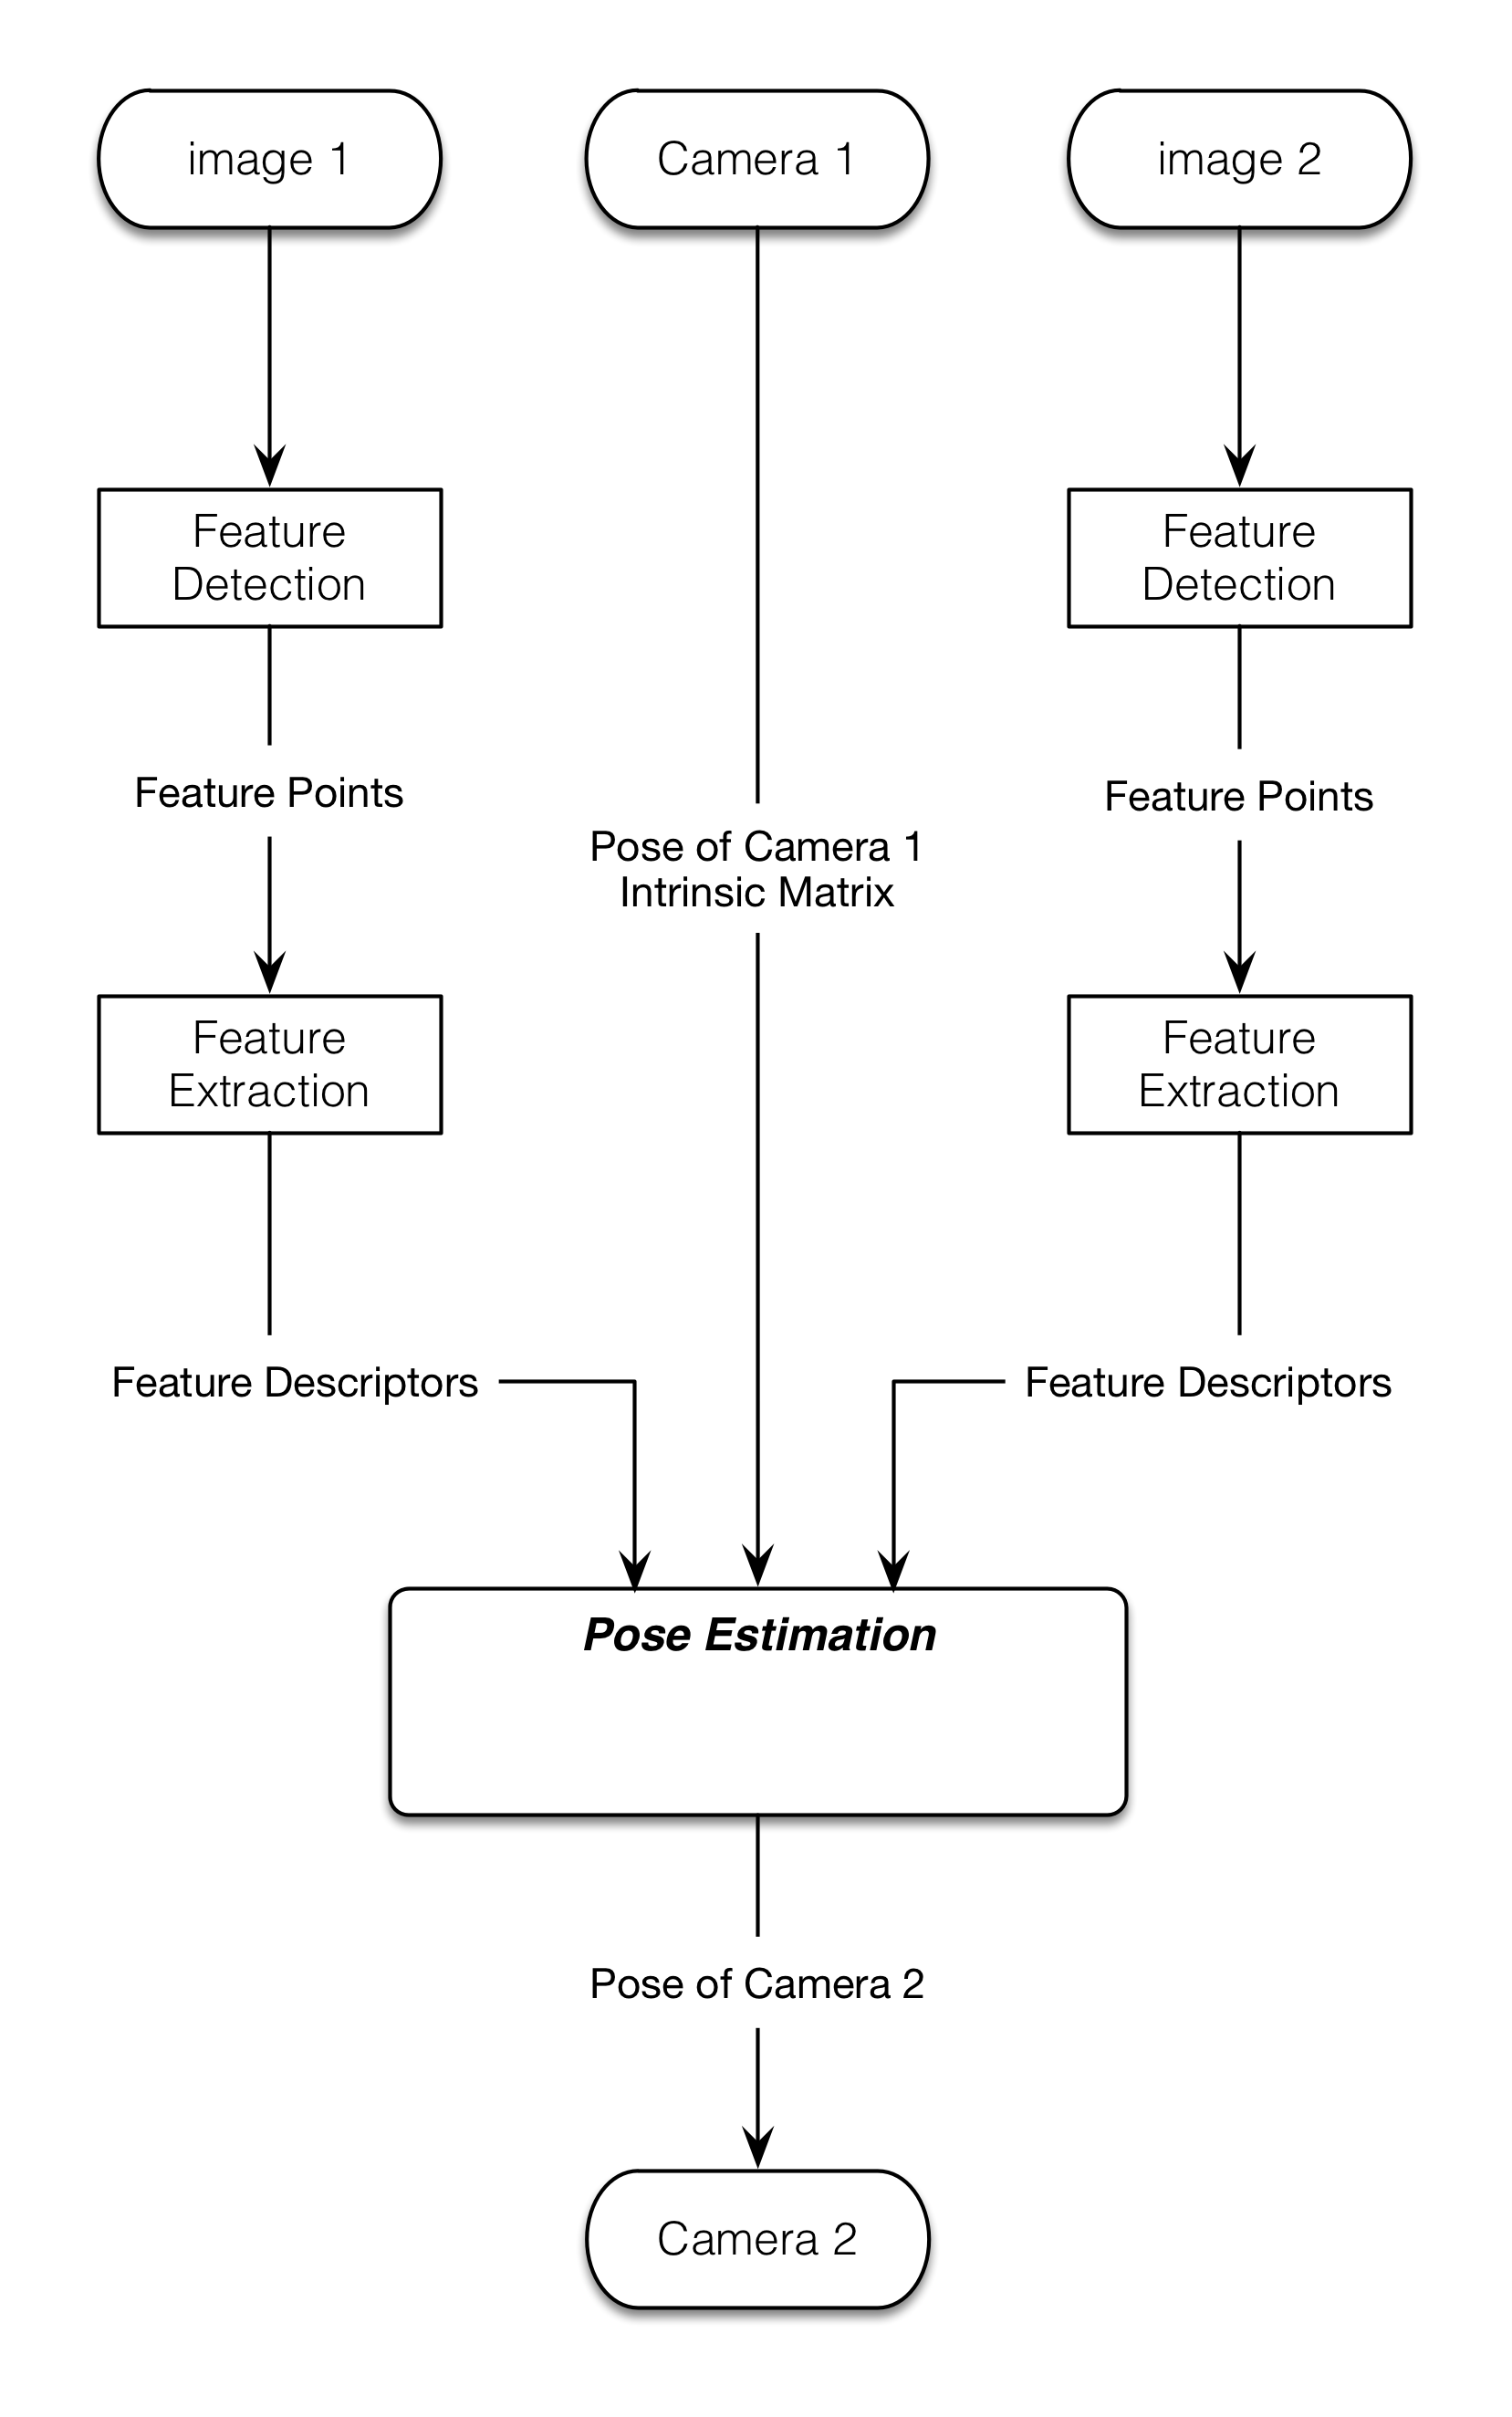
\includegraphics[width=75mm]{figures/pose_estimation_body} \\
(a) the body of planer pose estimation  & (b) entry requirements \\[6pt]
\end{tabular}
\caption{The concept of the planer pose estimation}\label{fig:pose_estimation}
\end{figure}

\section{PnP Problem} \label{sec:PnP_problem}
Determining the orientation and translation of a fully calibrated camera with respect to a known 3D model by using n (n>3) 3D points and their image projection is a classical problem in computer vision that is known as the perspective-n-point (PnP) problem. Schweighofer et al. \cite{schweighofer2006robust} represented the PnP problem as a multi model reprojection error function (cost function) with two local minima. One classical solution for this problem is using the Levenberg–Marquardt to minimize this cost function. In general, there are several ways to solve this problem based on the number of the given 3D points. For instance P3P, P4P and P5P. \\
The minimal P3P problem has been properly solved leading to many prominent linear solvers. Generally for PnP problem, currently several excellent noniterative $O(n)$ solutions have been proposed. EPnP \cite{lepetit2009epnp} tries to express all 3D points into the linear combination of four virtual control points, and approximately solve the resulting multivariate polynomial system using linearizion. The other well-known approach in this case is direct linear transformation (DLT) \cite{hartley2003multiple}. First it identifies the projection matrix and then extracts the calibration parameters and the camera pose. \\
Zheng et.al \cite{zheng2013revisiting} listed some PnP solutions that rely on the minimization of reprojection error. For the first time, Uymeyama \cite{umeyama1991least} introduced a linear method for optimization. The work tried to avoid local minimum by relaxing the PnP problem into a semidefinite program. The used memory due to relaxation was not efficient. After that, a direct least square (DLS) method was introduced by Hesch and Roumeliotis \cite{hesch2011direct} with the time complexity $O(n)$. This technique solves the drawback of Uymeyama method by solving the polynomial system.\\
\autoref{fig:pnp_sample} \footnote{\url{http://docs.opencv.org/trunk/doc/tutorials/calib3d/real_time_pose/real_time_pose.html}} shows the concept of PnP problem and the rotation and translation between the scene and the camera.

\begin{figure}[H]
  \centering
  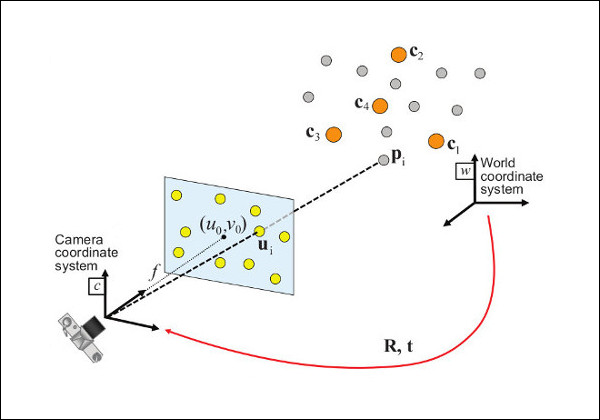
\includegraphics[width=140mm]{figures/pnp}
  \caption{PnP problem: Finding the pose of camera relative to the world coordinate \footnote{\url{http://docs.opencv.org/trunk/doc/tutorials/calib3d/real_time_pose/real_time_pose.html}} \label{fig:pnp_sample}
\end{figure}


\section{Tracking and Mapping}
This section explains the operation of the feature point-based tracking system. The tracking phase receives the input images and estimate the pose of camera relative to the scene. For tracking of each frame, the PnP solution is used to find out the rotation and translation of camera. In the following we will describe our novel approach that groups the input frames into some small packages that is called bundle. The pose of camera is estimated for all frames of the bundle efficiently and robustly. The 3D world model also is computed and updated at the end of the bundle processing.

\subsection{The bundle concept}
As already was mentioned in previous chapters, there are many approaches for feature point-based tracking. PTAM \cite{klein2007parallel} is a well-known approach for tracking the pose in AR workspace. The important point of this technique is that the tracking and mapping are separated and run in two parallel threads. In the case of mapping phase, the obtained 3D world map is optimized by a bundle adjustment after each new frame. The result of bundle adjustment for the market-based tracking in Ubitrack illustrates that the noisy data including the noise in images and also mismatch in matches vector have a negative effect on that.\\
Based on our experience about the result of bundle adjustment for the marker-based tracking (\autoref{subsec:result_ba}), we decided to use the bundle adjustment for a group of images instead of two or three images. For this purpose and after of several tests over the result of bundle adjustment, the input frames are grouped into the same small packages, usually five frames, that is called a bundle. The size of the bundle is a parameters in our approach and we called it local threshold. Based on our evaluation (shown in \autoref{sec:local_threshold}) 5 is the best value for local threshold.\\
The feature points of each frame are extracted by A-KAZE feature detection and extraction. After that the robust feature matching is applied to filter out the outliers between the robust feature points of previous frames (***REFRENCE To SECTION***) and new frame. For instance for a bundle with size five frames we execute the robust feature matching four times: between the first and the second; the resulting roust feature points with the third frames; the resulting roust feature points with the forth frames; and finally the resulting robust feature points from all previous matching with the fifth frame. \\
% TODO: Image
 After this step a recursive function is used to identify the feature points that are available in all frames of a bundle. These feature points are called the elite feature point. The 3D points are reconstructed by using the elite feature points of each bundle and the pose of the corresponding cameras. After that, the pose of each camera is optimized by a non-planner pose optimization (PnP solution) to enhance the rotation and translation matrices based on the resulting 3D points.A cvsba bundle adjustment with the type Sba::STRUCTURE (local bundle adjustment) is applied to refine the 3D points based on the new camera poses. The final 3D points are added to or updated in the 3D world Map.\\
\autoref{fig:bundle_concept} illustrates a schematic view (data flow) of our bundle concept.

\begin{figure}[H]
  \centering
  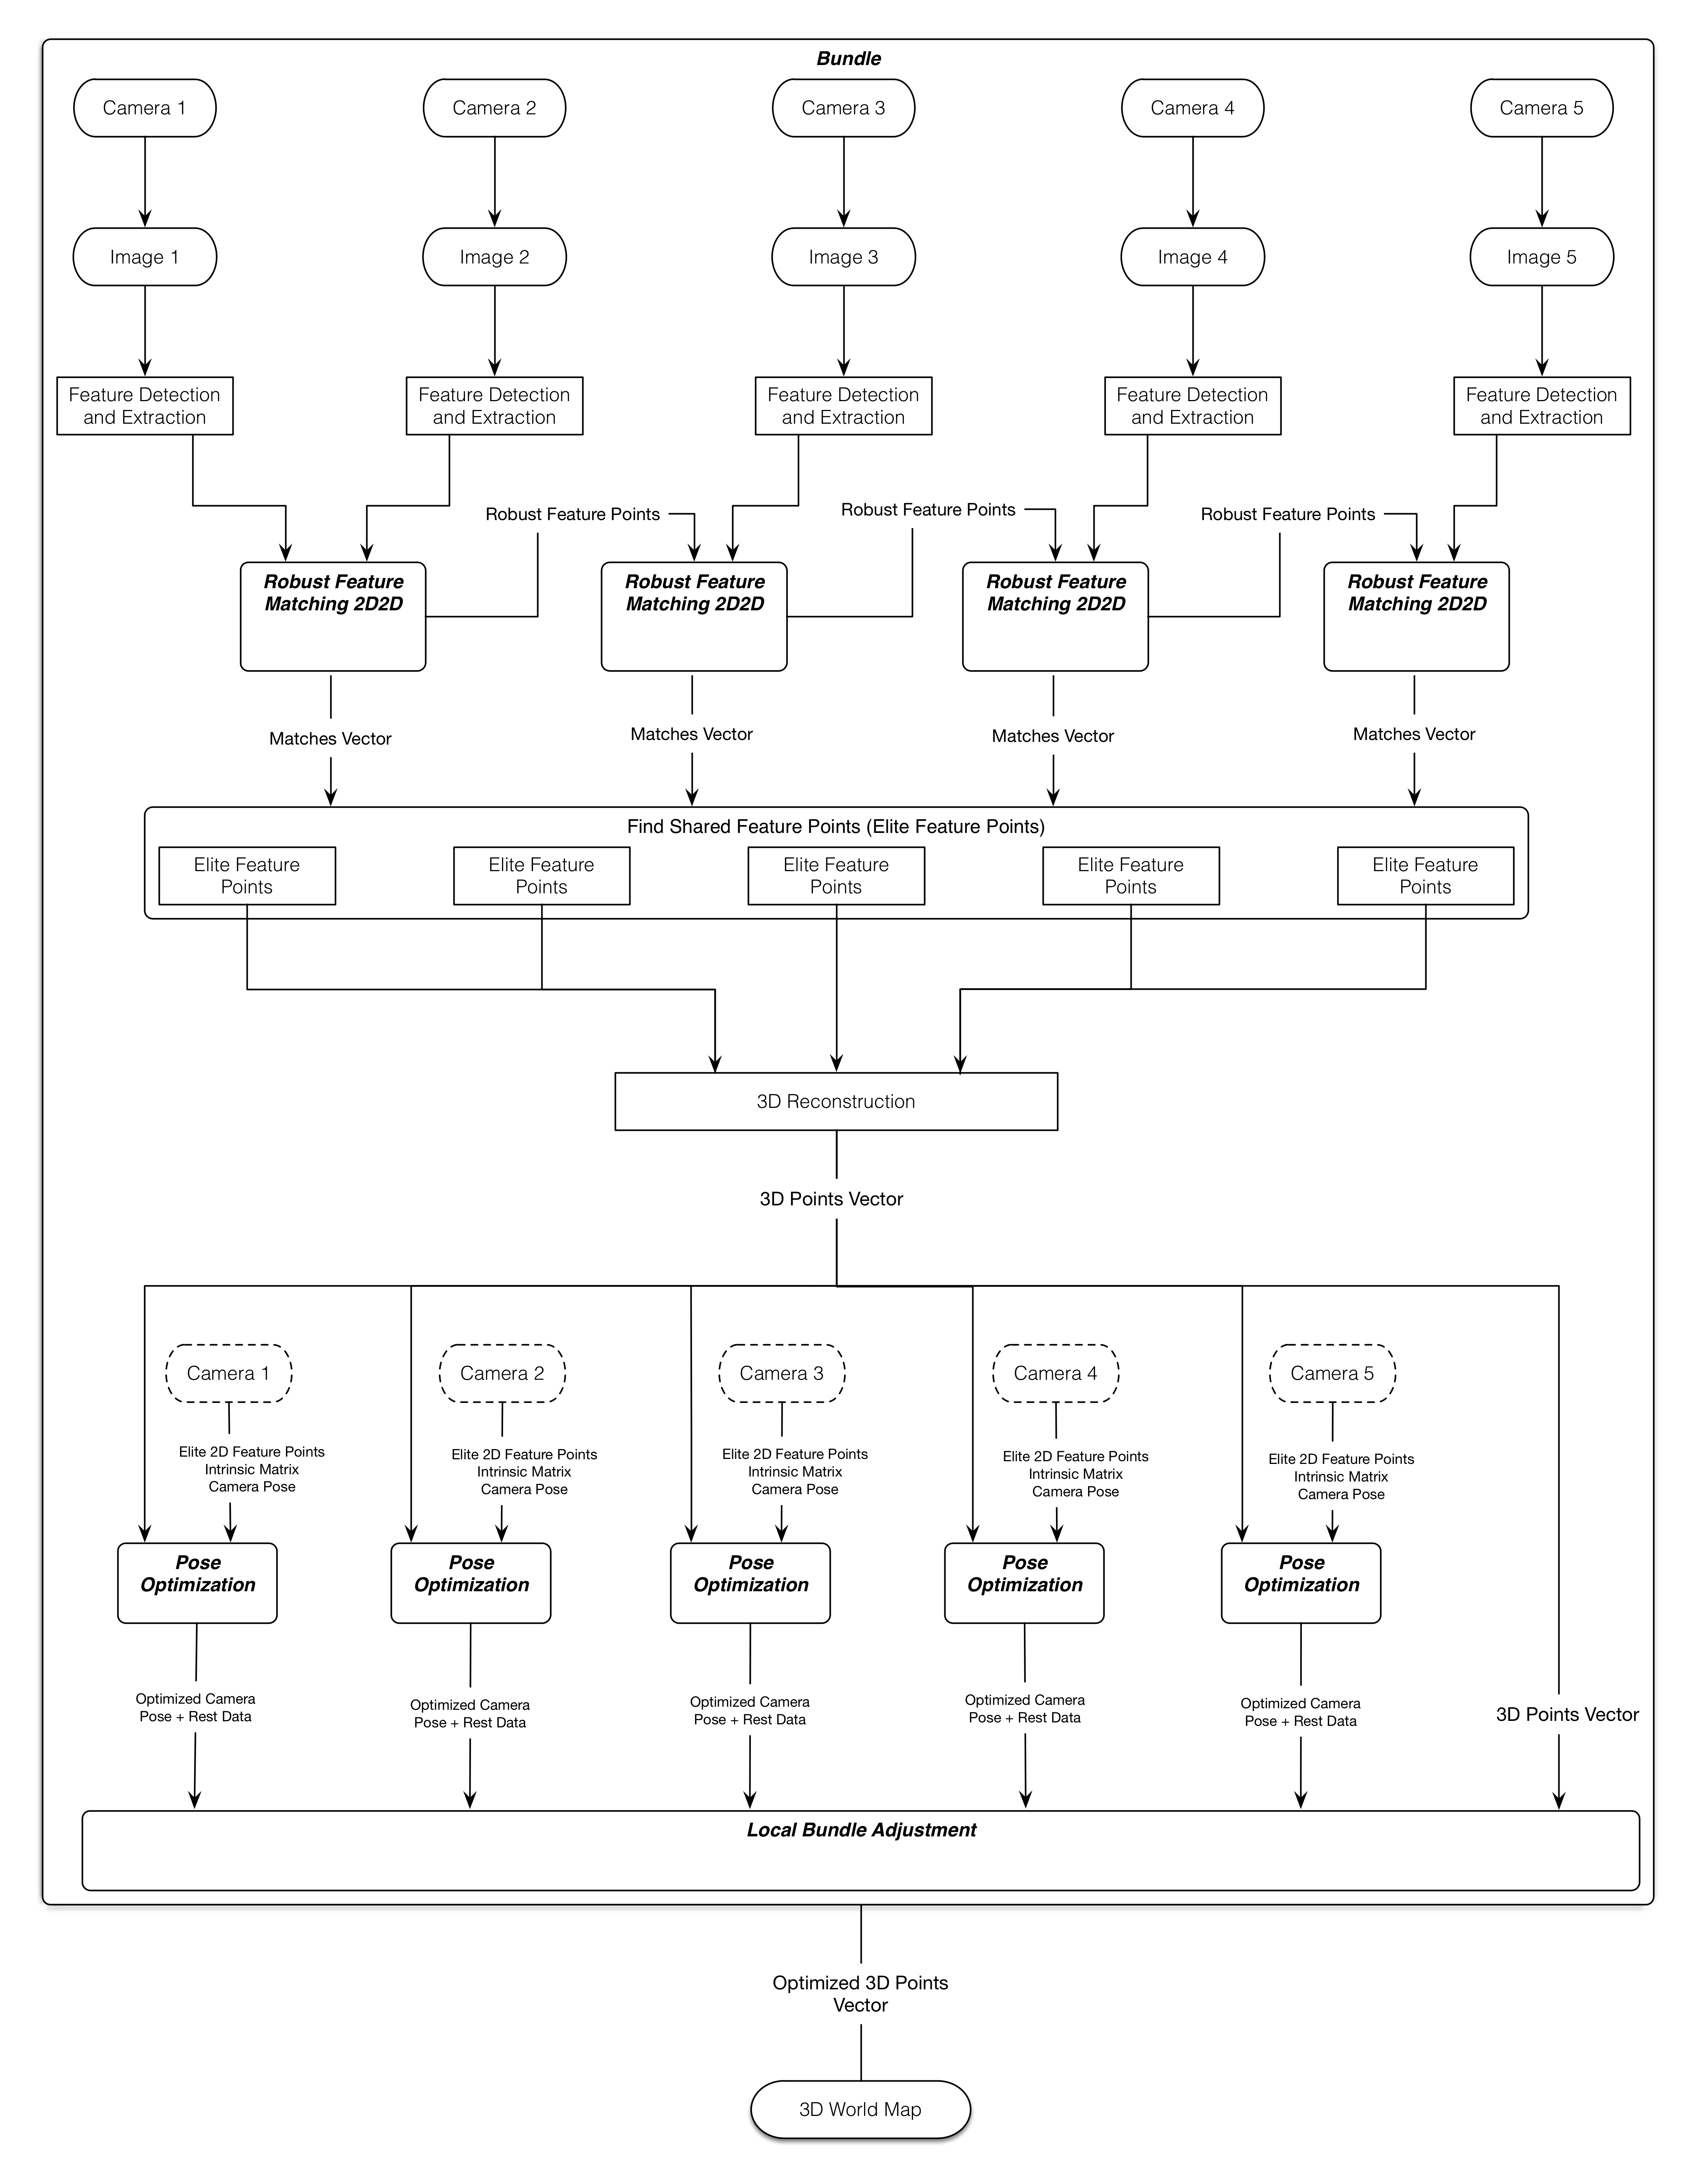
\includegraphics[width=\textwidth, height=\textheight, keepaspectratio]{figures/bundle_concept}
  \caption{The data flow of the bundle concept}\label{fig:bundle_concept}
\end{figure}

\subsection{Pose estimation for the first bundle}\label{subsec:pose_first_bundle}
Based on the new bundle concept that was introduced in previous section, all input frames are grouped into five frames and are processed independent of other bundles. In this section, we describe the operations that are necessary for first bundle.\\
First of all, we need to determine a prior estimation for the pose of each camera for the 3D reconstruction. Two approaches are considered to compute the initiate pose for each camera inside a bundle. They are listed as follows:
\begin{enumerate}
\item Initiate pose from the reference system: the pose of all cameras are provided by the reference system.
\item Initiate pose estimation by planner tracking: in this method the pose of the first camera is taken from the pose system and converted to the corresponding homography matrix. The pose of the rest cameras are computed consequently relying on the approach that was explained in \autoref{subsec:pose_estimation_planer_tracking}.
\end{enumerate}
Based on a comparison between these two approaches that will be presented in \autoref{sec:refrence_system}, the first approach is selected for the initiate estimation of camera poses.\\
As described in previous section, we use the A-KAZE feature detection and extraction along with a a recursive technique to find the elite feature points of a bundle. \\
 For this purpose, we begin from the features of the first and the second frames are matched by a robust feature matching 2D 2D. The output result is a matches vector and a robust feature points (\autoref{subsec:robust_feature_matching_2D_2D}). The outcome robust feature points is a vector of feature points from the second frame, where their feature descriptors are agreement between the both images. The robust feature points between the first and the second frames are matched by another robust feature matching 2D 2D and the new feature points of third frame. This operation is continued consequently for all five frames of this bundle. The final result is a vector of feature points from the last frame (fifth frame) that its feature descriptors are agreement in all five frames. Right now it is the time to select the correspondence elite feature points in the first, second, third and forth frames. Thus we begin from down to up. The matches vector from the last robust feature matching is used to obtain the indices of the elite feature points of forth frame. The rest matches vector also are applied consecutively to obtain the elite feature points of the first, second and third frames. Finally, we have five elite feature points with the same size that their feature points are matched by the robust feature matching. There are mostly close and precise and good data points for 3D reconstruction.\\
 % TODO: (SHOW A PICTURE)
The elite feature points and the camera pose of all frames are gathered to reconstruct the first 3D set of our environment.
in Ubitrack, the \detokenize{Algorithm::get3DPositionWithResidual()} function is used for reconstruction. The size of these 3D points are as same as the size of the elite feature points of each camera. In this thesis, because in future we need to compare the 3D points with 2D points, the feature descriptor of 2D point (not matter from which frame, the feature descriptors for all frames are closely similar) is allocated to correspondence 3D point as a measure parameter for comparing a 2D and 3D point. After that, a non-planner pose optimization function which was implemented in UBitrack as the name \detokenize{Ubitrack::Algorithm::PoseEstimation2D3D::optimizePose()} is used to optimized the pose of each camera by using a robust feature matching 2D 3D between the new obtained 3D points and elite feature points of each frame. This function was developed based on a non-planer approach for pose estimation that was proposed in \cite{lu2000fast}.\\
\autoref{fig:pose_optimization} demonstrates a schematic view of our pose optimization.
\begin{figure}[H]
  \centering
  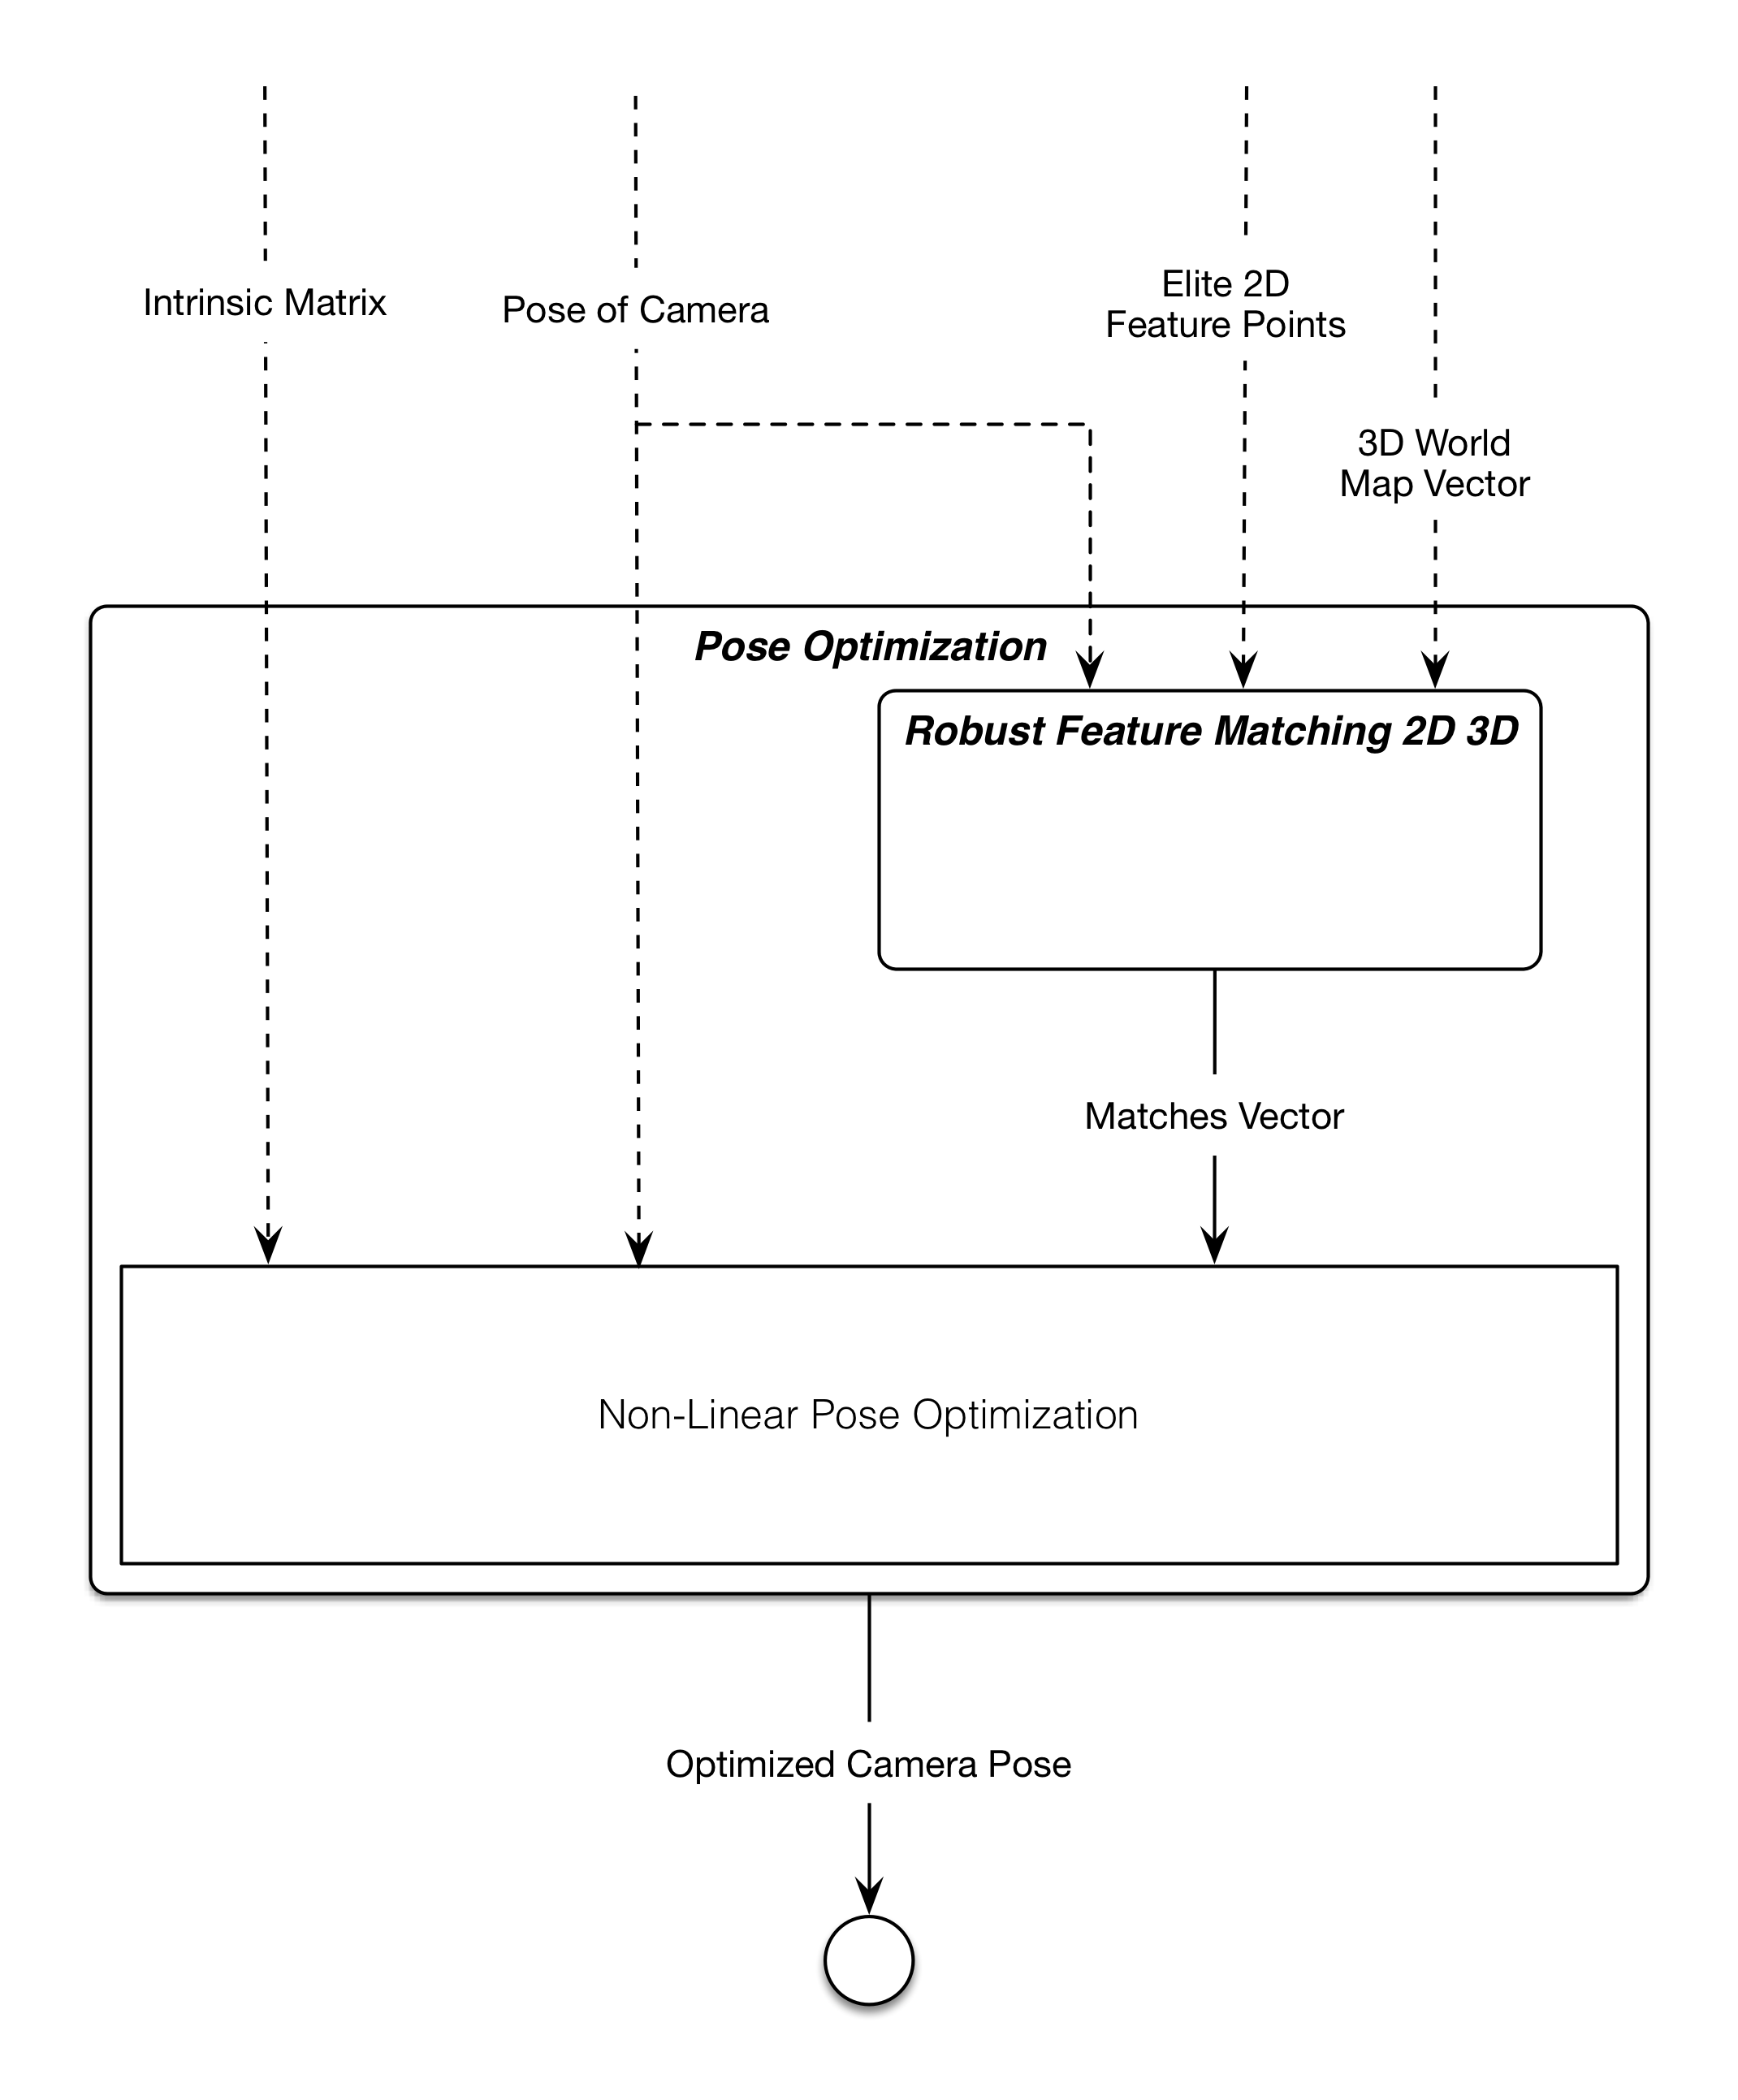
\includegraphics[width=100mm]{figures/pose_optimization}
  \caption{The data flow of pose optimization}\label{fig:pose_optimization}
\end{figure}

For the last step of this scenario, a bundle adjustment is exploited to refine the 3D points as much as we can. The necessary parameters including: the elite feature points of all frames, the optimized camera poses, the first estimation of 3D points and the intrinsic of all cameras are gathered in the Ubitrack bundle adjustment (structure type \autoref{subsec:type_of_optimization}) to optimize the 3D points. The number of iteration is 300 and the minimum of reprojection error is $1\mbox{\textsc{e}}-10$. The final optimized 3D points are added to 3D world map vector. The operation of the first bundle is finished here.

\subsection{Pose estimation for the second bundle} \label{subsec:pose_second_bundle}
The scenario for processing the second bundle is a little bit different with the first bundle. In the first bundle, the initiate or prior pose have been taken from the reference system whereas the pose estimation of the second bundle's frames are computed by two parts:
\begin{enumerate}
\item The prior pose estimation of each camera are computed by the planner tracking (see \autoref{subsec:pose_estimation_planer_tracking}). For instance the pose of sixth camera is computed by the homography matrix between the fifth camera and the sixth camera. The pose of other cameras also are determined by this technique sequentially. 
\item The points in 3D world map are projected into the image according to the frame's prior pose estimated. The camera pose is updated by these match 3D and 2D points.
\end{enumerate}

\autoref{fig:pose_estimation_optimization} demonstrates the two steps of pose estimation. The first step is done by planner tracking technique and the second step by pose optimization.

\begin{figure}[H]
  \centering
  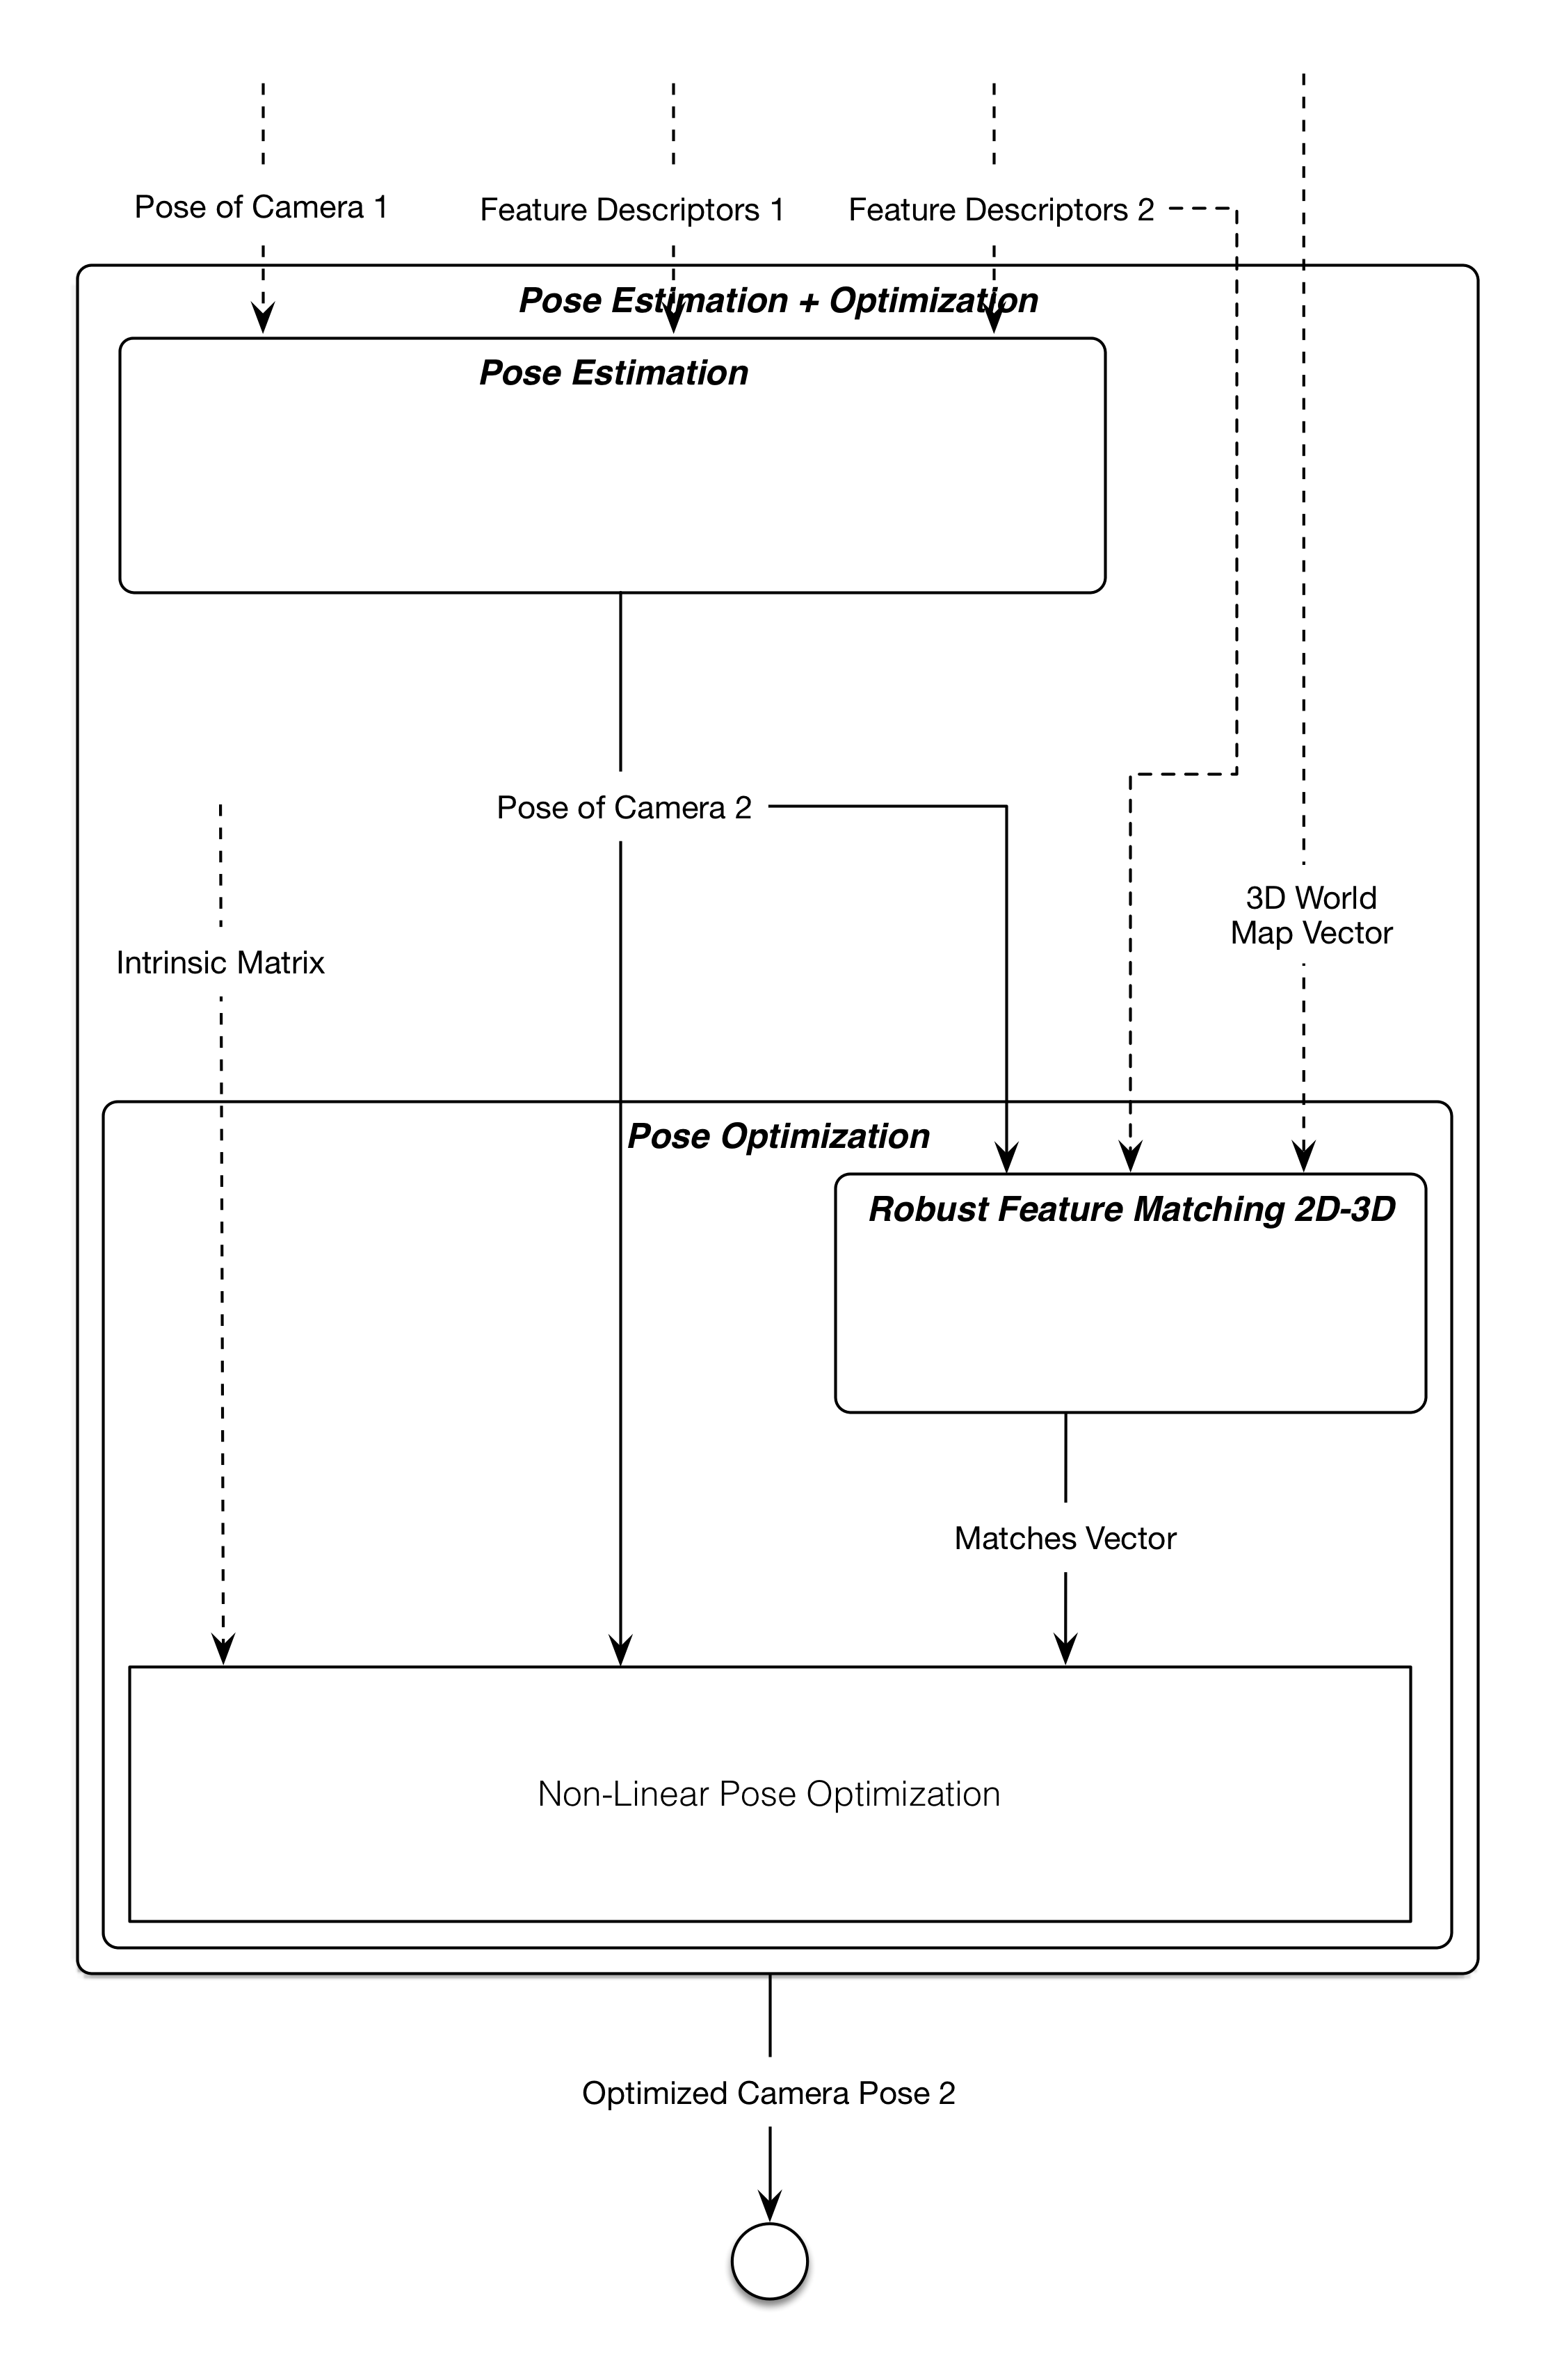
\includegraphics[width=100mm]{figures/pose_estimation_optimization}
  \caption{two steps of pose estimation by using the 3D world map}\label{fig:pose_estimation_optimization}
\end{figure}

The rest operation including: feature extraction, robust feature matching, recursive approach for finding the elite feature points, 3D reconstruction and the local bundle adjustment are exactly the same as the first bundle. 

\begin{figure}[H]
  \centering
  \includegraphics[angle=90, height=\textheight, keepaspectratio]{figures/bundle_second}
  \caption{The data flow of two connected bundles}\label{fig:bundle_second}
\end{figure}

\subsection{Update 3D points (world map)} \label{subsec:update_3d_points}
At the end of each bundle, a set of 3D points are reconstructed. After that, we need to update the 3D world map vector based on these new 3D points. In this thesis, instead of adding the new 3D points to the world map after the each bundle and growing the 3D model of world that is usual in SLAM methods, we just keep the 3D points that are the same as the 3D world map. In more detail, for the first bundle the optimized 3D points directly store into the 3D world map. For the second one, the new optimized 3D points are compared with the 3D world map vector. For this purpose, both 3D sets are projected to the last frame of the last bundle and are compared by a robust feature matching 3D 3D based on their feature descriptors. The new 3D world map is updated by these common 3D points. The size of new 3D world map also drops because we just the common 3D points are considered and the new points ignored.
In the next step, a bundle adjustment (global bundle adjustment) is applied to refine these 3D points. For global bundle adjustment we need the 2D elite feature points that reconstructed the new 3D world map but matching the indexes of these 3D points and their 2D points is very complicated. To solve this problem, a big data table is used to save the correct index matches between the each 3D points and their elite feature points after the local bundle adjustment.\\
Regarding to this fact that the corresponding elite feature points of each 3D point right now is known in our data table, the new 3D points are optimized by the global bundle adjustment. The \autoref{fig:global_bundle_adjustment} show an overall view of the global bundle adjustment after the processing of the second bundle.

\begin{figure}[H]
  \centering
  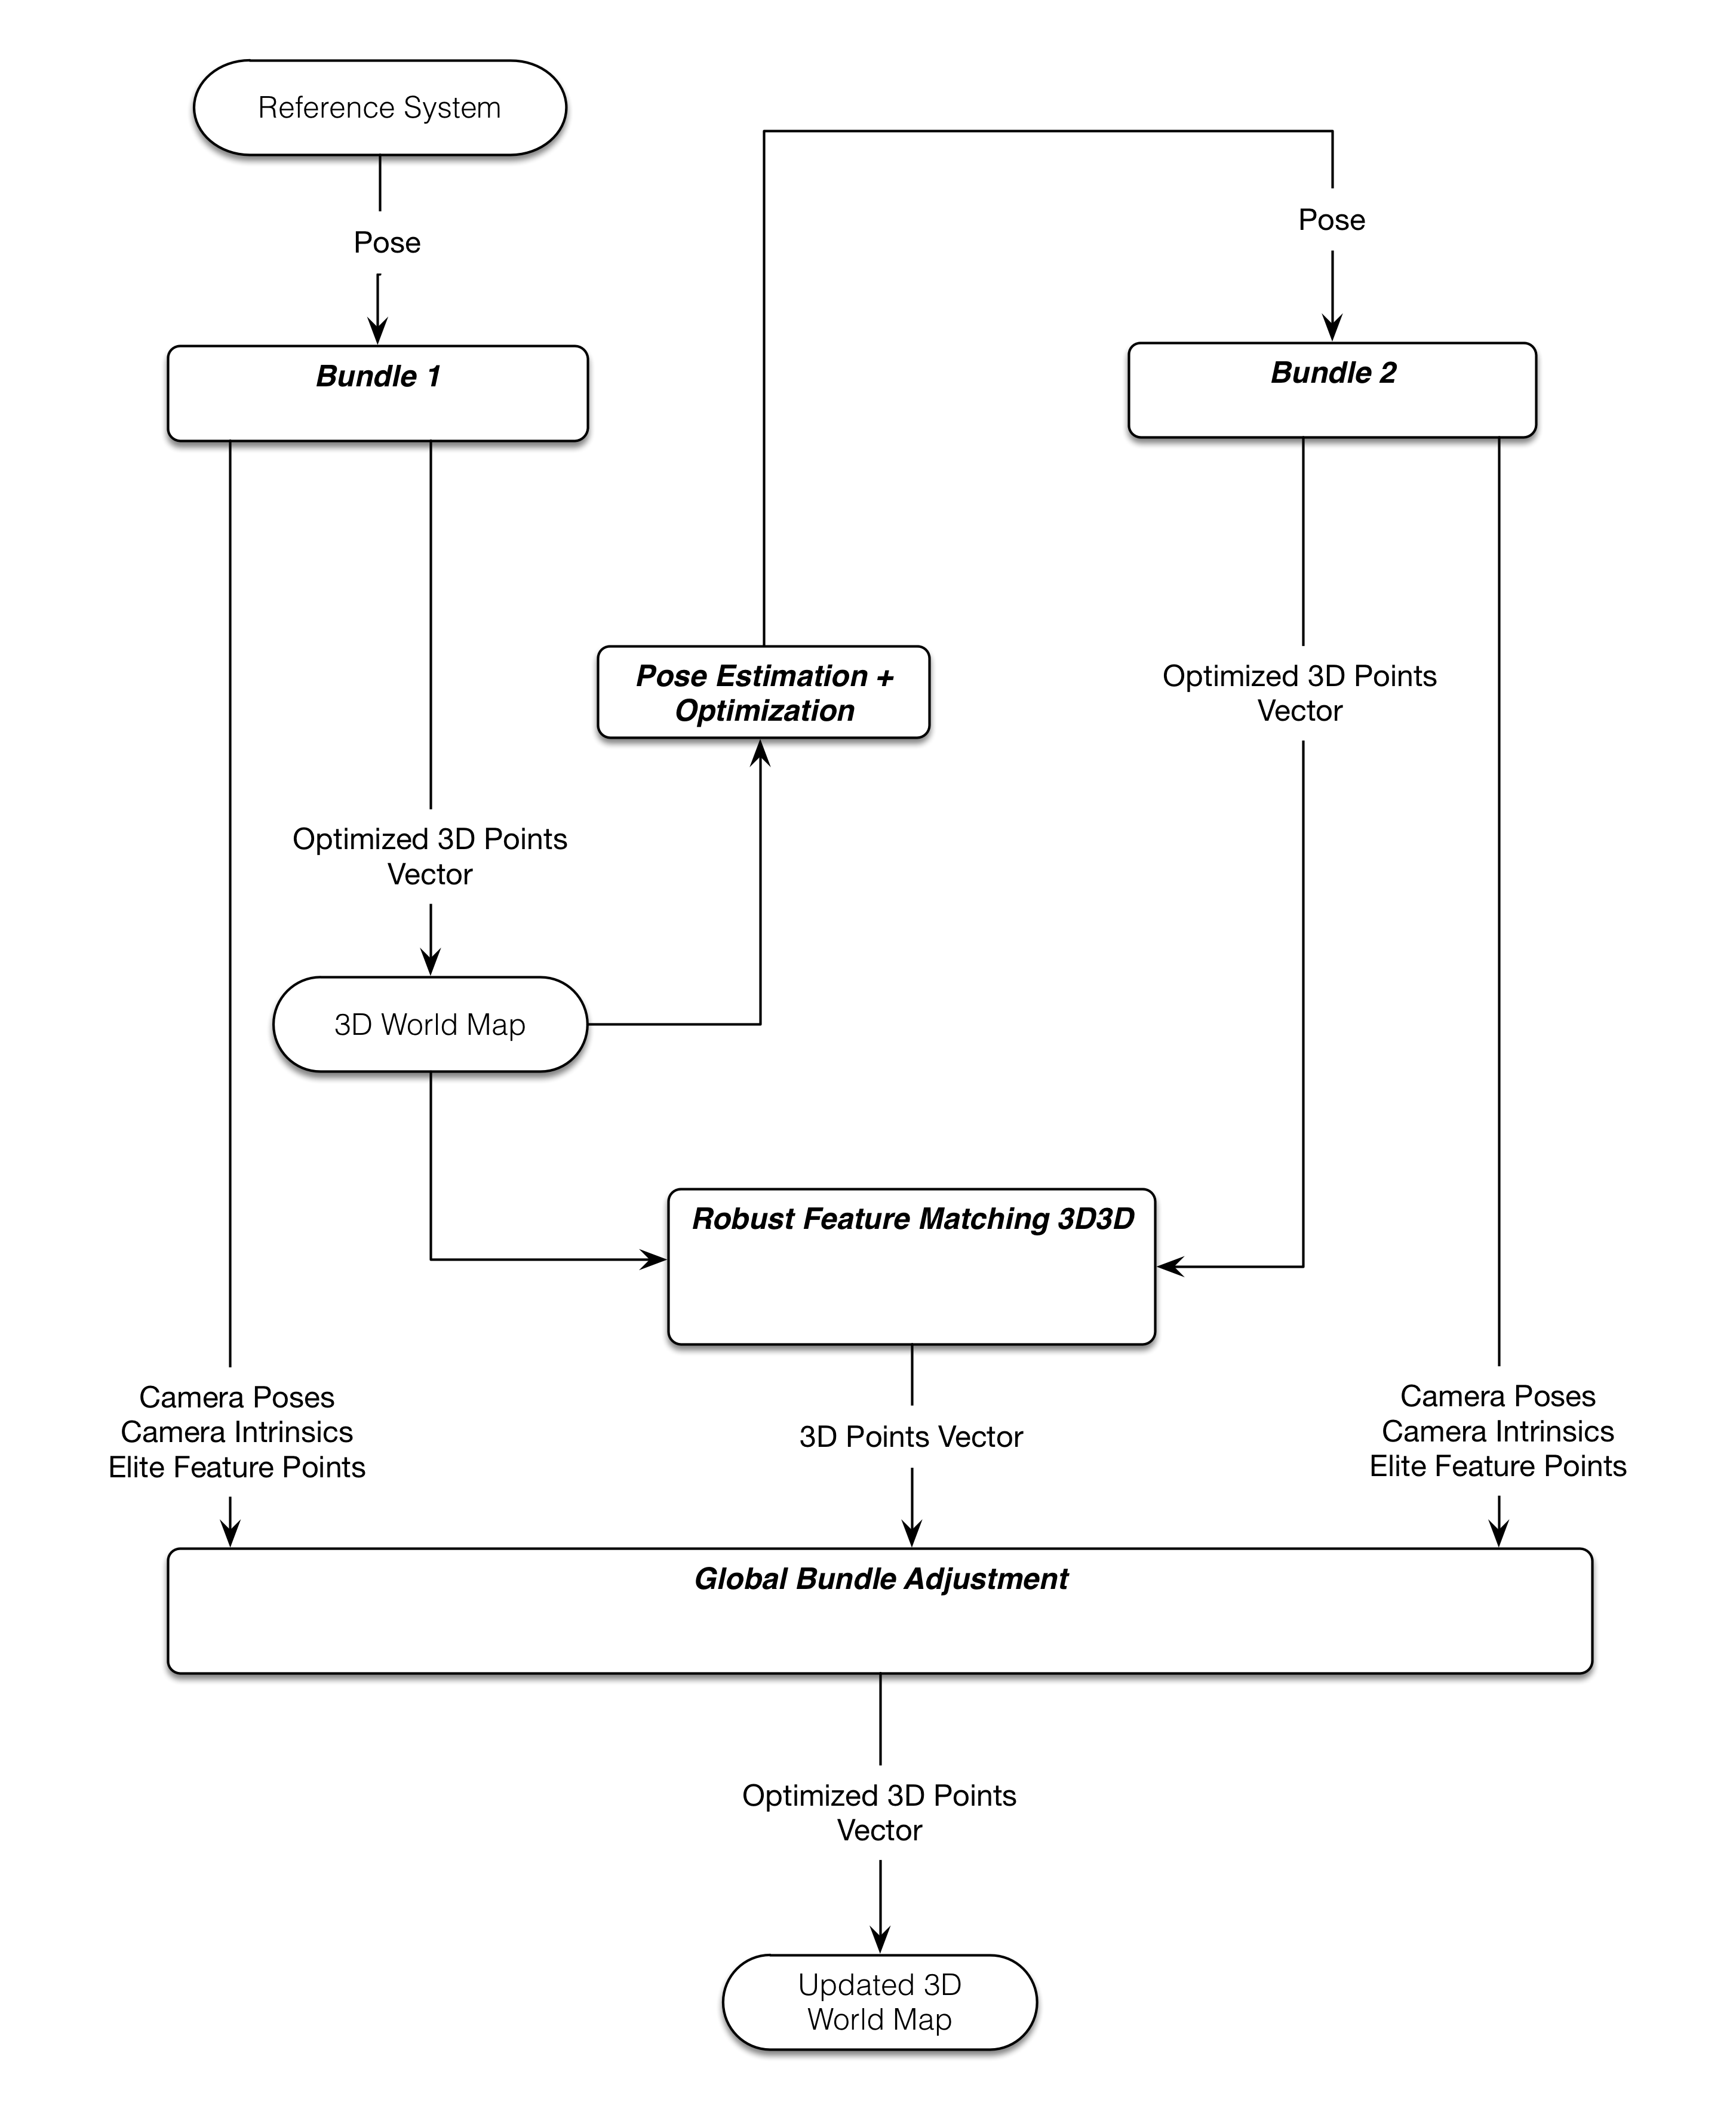
\includegraphics[width=120mm]{figures/global_bundle_adjustment}
  \caption{global bundle adjustment after the second bundle}\label{fig:global_bundle_adjustment}
\end{figure}

As was introduced, the 3D points were remained in world map which robustly matched with the new points. Keeping the robust matched points causes the size of world map decreases after each bundle and after a long time (more than 5 bundles) the remain 3D in our world map are not sufficient for mapping phase and pose estimation of the new frame. To prevent of this issue, after each four bundles (20 frames), instead of updating the 3D world map, we just keep the 3D points that are directly computed by local bundle adjustment. For instance, the 3D points of first, second, third and forth bundle are updated by a robust feature matching 3D 3D and global bundle adjustment. But for the fifth bundle, because the size of 3D world map is not enough (usually less than 100 points), the 3D world map is replaced by the new 3D points after the local bundle adjustment directly. This cycle is repeated after processing of each four bundles. The \autoref{fig:mapping_concept} illustrates the updating of 3D world map after five bundles.

\begin{figure}[H]
  \centering
  \includegraphics[width=150mm]{figures/mapping}
  \caption{The value of 3D world map vector after the five bundles}\label{fig:mapping_concept}
\end{figure}

In this chapter, we introduced a novel feature-based pose estimation approach. The input frames are grouped into bundles and the 3D points of each bundle are reconstructed based on a four layer robust feature matching and bundle adjustment. The 3D points also are updated rely on the fact that just keep the 3D points that are common in both 3D data sets. The 3D world map is refreshed with the new 3D points directly after each five bundles. In the next chapter we will show the result of this innovative approach and compare with the result of marker-based pose estimation, which was implemented in Ubitarck, on the same scenario and data frames.
